%package list
\documentclass{article}
\usepackage[top=3cm, bottom=3cm, outer=3cm, inner=3cm]{geometry}
\usepackage{multicol}
\usepackage{graphicx}
\usepackage{url}
%\usepackage{cite}
\usepackage{hyperref}
\usepackage{array}
%\usepackage{multicol}
\newcolumntype{x}[1]{>{\centering\arraybackslash\hspace{0pt}}p{#1}}
\usepackage{natbib}
\usepackage{pdfpages}
\usepackage{multirow}
\usepackage[normalem]{ulem}
\useunder{\uline}{\ul}{}
\usepackage{svg}
\usepackage{xcolor}
\usepackage{listings}
\lstdefinestyle{ascii-tree}{
    literate={├}{|}1 {─}{--}1 {└}{+}1 
  }
\lstset{basicstyle=\ttfamily,
  showstringspaces=false,
  commentstyle=\color{red},
  keywordstyle=\color{blue}
}
%\usepackage{booktabs}
\usepackage{caption}
\usepackage{subcaption}
\usepackage{float}
\usepackage{array}

\newcolumntype{M}[1]{>{\centering\arraybackslash}m{#1}}
\newcolumntype{N}{@{}m{0pt}@{}}


%%%%%%%%%%%%%%%%%%%%%%%%%%%%%%%%%%%%%%%%%%%%%%%%%%%%%%%%%%%%%%%%%%%%%%%%%%%%
%%%%%%%%%%%%%%%%%%%%%%%%%%%%%%%%%%%%%%%%%%%%%%%%%%%%%%%%%%%%%%%%%%%%%%%%%%%%
\newcommand{\itemEmail}{rvaldiviase@unsa.edu.pe}
\newcommand{\itemStudent}{Ryan Fabian Valdivia Segovia}
\newcommand{\itemCourse}{Fundamentos de la programación 2}
\newcommand{\itemCourseCode}{1701213}
\newcommand{\itemSemester}{II}
\newcommand{\itemUniversity}{Universidad Nacional de San Agustín de Arequipa}
\newcommand{\itemFaculty}{Facultad de Ingeniería de Producción y Servicios}
\newcommand{\itemDepartment}{Departamento Académico de Ingeniería de Sistemas e Informática}
\newcommand{\itemSchool}{Escuela Profesional de Ingeniería de Sistemas}
\newcommand{\itemAcademic}{2023 - B}
\newcommand{\itemInput}{Del 08 de Enero 2023}
\newcommand{\itemOutput}{Al 15 de Enero 2023}
\newcommand{\itemPracticeNumber}{20}
\newcommand{\itemTheme}{Miembros de clase}
%%%%%%%%%%%%%%%%%%%%%%%%%%%%%%%%%%%%%%%%%%%%%%%%%%%%%%%%%%%%%%%%%%%%%%%%%%%%
%%%%%%%%%%%%%%%%%%%%%%%%%%%%%%%%%%%%%%%%%%%%%%%%%%%%%%%%%%%%%%%%%%%%%%%%%%%%

\usepackage[english,spanish]{babel}
\usepackage[utf8]{inputenc}
\AtBeginDocument{\selectlanguage{spanish}}
\renewcommand{\figurename}{Figura}
\renewcommand{\refname}{Referencias}
\renewcommand{\tablename}{Tabla} %esto no funciona cuando se usa babel
\AtBeginDocument{%
	\renewcommand\tablename{Tabla}
}

\usepackage{fancyhdr}
\pagestyle{fancy}
\fancyhf{}
\setlength{\headheight}{30pt}
\renewcommand{\headrulewidth}{1pt}
\renewcommand{\footrulewidth}{1pt}
\fancyhead[L]{\raisebox{-0.2\height}{
\includegraphics[width=3cm]{img/logo_episunsa.png}}}
\fancyhead[C]{\fontsize{7}{7}\selectfont	\itemUniversity \\ \itemFaculty \\ \itemDepartment \\ \itemSchool \\ \textbf{\itemCourse}}
\fancyhead[R]{\raisebox{-0.2\height}{
\includegraphics[width=1.2cm]{img/logo_abet}}}
\fancyfoot[L]{Estudiante Ryan Valdivia}
\fancyfoot[C]{\itemCourse}
\fancyfoot[R]{Página \thepage}

% para el codigo fuente
\usepackage{listings}
\usepackage{color, colortbl}
\definecolor{dkgreen}{rgb}{0,0.6,0}
\definecolor{gray}{rgb}{0.5,0.5,0.5}
\definecolor{mauve}{rgb}{0.58,0,0.82}
\definecolor{codebackground}{rgb}{0.95, 0.95, 0.92}
\definecolor{tablebackground}{rgb}{0.8, 0, 0}

\lstset{frame=tb,
	language=bash,
	aboveskip=3mm,
	belowskip=3mm,
	showstringspaces=false,
	columns=flexible,
	basicstyle={\small\ttfamily},
	numbers=none,
	numberstyle=\tiny\color{gray},
	keywordstyle=\color{blue},
	commentstyle=\color{dkgreen},
	stringstyle=\color{mauve},
	breaklines=true,
	breakatwhitespace=true,
	tabsize=3,
	backgroundcolor= \color{codebackground},
}

\begin{document}
	
	\vspace*{10px}
	
	\begin{center}	
		\fontsize{17}{17} \textbf{ Informe de Laboratorio \itemPracticeNumber}
	\end{center}
	\centerline{\textbf{\Large Tema: \itemTheme}}
	%\vspace*{0.5cm}	

	\begin{flushright}
		\begin{tabular}{|M{2.5cm}|N|}
			\hline 
			\rowcolor{tablebackground}
			\color{white} \textbf{Nota}  \\
			\hline 
			     \\[30pt]
			\hline 			
		\end{tabular}
	\end{flushright}	

	\begin{table}[H]
		\begin{tabular}{|x{4.7cm}|x{4.8cm}|x{4.8cm}|}
			\hline 
			\rowcolor{tablebackground}
			\color{white} \textbf{Estudiante} & \color{white}\textbf{Escuela}  & \color{white}\textbf{Asignatura}   \\
			\hline 
			{\itemStudent \par \itemEmail} & \itemSchool & {\itemCourse \par Semestre: \itemSemester \par Código: \itemCourseCode}     \\
			\hline 			
		\end{tabular}
	\end{table}		
	
	\begin{table}[H]
		\begin{tabular}{|x{4.7cm}|x{4.8cm}|x{4.8cm}|}
			\hline 
			\rowcolor{tablebackground}
			\color{white}\textbf{Laboratorio} & \color{white}\textbf{Tema}  & \color{white}\textbf{Duración}   \\
			\hline 
			\itemPracticeNumber & \itemTheme & 04 horas   \\
			\hline 
		\end{tabular}
	\end{table}
	
	\begin{table}[H]
		\begin{tabular}{|x{4.7cm}|x{4.8cm}|x{4.8cm}|}
			\hline 
			\rowcolor{tablebackground}
			\color{white}\textbf{Semestre académico} & \color{white}\textbf{Fecha de inicio}  & \color{white}\textbf{Fecha de entrega}   \\
			\hline 
			\itemAcademic & \itemInput &  \itemOutput  \\
			\hline 
		\end{tabular}
	\end{table}
	
	\section{Tarea}
	\begin{itemize}
			\item Crear diagrama de clases UML y programa.
			\item Crear los miembros de cada clase de la forma más adecuada: como miembros de clase o de instancia.
			\item Crear la clase Mapa, que esté constituida por el tablero antes visto, que posicione soldados en ciertas posiciones aleatorias (entre 1 y 10 soldados por cada ejército, sólo 1 ejército por reino). Se deben generar ejércitos de 2 reinos.
No se admite guerra civil. El Mapa tiene como atributo el tipo de territorio que es (bosque, campo abierto, montaña, desierto, playa). La cantidad de soldados, así como todos sus atributos se deben generar aleatoriamente.
			\item Dibujar el Mapa con las restricciones que sólo 1 soldado como máximo en cada cuadrado.
			\item El mapa tiene un solo tipo de territorio.
			\item Considerar que el territorio influye en los resultados de las batallas, así cada reino tiene bonus según el territorio: Inglaterra - bosque, Francia - campo abierto, Castilla-Aragón - montaña, Moros - desierto, Sacro Imperio Romano-Germánico - bosque, playa, campo abierto. En dichos casos, se aumenta el nivel de vida en 1 a todos los soldados del reino beneficiado.
			\item En la historia, los ejércitos estaban conformados por diferentes tipos de soldados, que tenían similitudes, pero también particularidades.
			\item Basándose en la clase Soldado crear las clases Espadachín, Arquero, Caballero y Lancero. Las cuatro clases heredan de la superclase Soldado pero aumentan atributos y métodos, o sobrescriben métodos heredados.
			\item Los espadachines tienen como atributo particular "longitud de espada" y como acción "crear un muro de escudos" que es un tipo de defensa en particular.
			\item Los caballeros pueden alternar sus armas entre espada y lanza, además de desmontar (sólo se realiza cuando está montando e implica defender y cambiar de arma a espada), montar (sólo se realiza cuando está desmontado e implica montar, cambiar de arma a lanza y envestir). El caballero también puede envestir, ya sea montando o desmontando, cuando es desmontado equivale a atacar 2 veces pero cuando está montando implica a atacar 3 veces.
			\item Los arqueros tienen un número de flechas disponibles las cuales pueden dispararse y se gastan cuando se hace eso.
			\item Los lanceros tienen como atributo particular, "longitud de lanza" y como acción "schiltrom" (como una falange que es un tipo de defensa en particular y que aumenta su nivel de defensa en 1).
			\item Tendrá 2 Ejércitos que pueden ser constituidos sólo por espadachines, caballeros, arqueros y lanceros. No se acepta guerra civil. Crear una estructura de datos conveniente para el tablero. Los soldados del primer ejército se almacenarán en un arreglo estándar y los soldados del segundo ejército se almacenarán en un ArrayList. Cada soldado tendrá un nombre autogenerado: Espadachin0X1, Arquero1X1, Caballero2X2, etc., un valor de nivel de vida autogenerado aleatoriamente, la fila y columna también autogenerados aleatoriamente (no puede haber 2 soldados en el mismo cuadrado) y valores autogenerados para el resto de atributos.
			\item Todos los caballeros tendrán los siguientes valores: ataque 13, defensa 7, nivel
de vida [10..12] (el nivel de vida actual empieza con el valor del nivel de vida).
			\item Todos los arqueros tendrán los siguientes valores: ataque 7, defensa 3, nivel
de vida [3..5] (el nivel de vida actual empieza con el valor del nivel de vida).
			\item Todos los espadachines tendrán los siguientes valores: ataque 10, defensa 8,
nivel de vida [8..10] (el nivel de vida actual empieza con el valor del nivel de
vida).
			\item Todos los lanceros tendrán los siguientes valores: ataque 5, defensa 10, nivel
de vida [5..8] (el nivel de vida actual empieza con el valor del nivel de vida).
			\item Mostrar el tablero, distinguiendo los ejércitos y los tipos de soldados creados.
Además, se debe mostrar todos los datos de todos los soldados creados para
ambos ejércitos. Además de los datos del soldado con mayor vida de cada
ejército, el promedio de nivel de vida de todos los soldados creados por ejército,
los datos de todos los soldados por ejército en el orden que fueron creados y

un ranking de poder de todos los soldados creados por ejército (del que tiene
más nivel de vida al que tiene menos) usando algún algoritmo de ordenamiento.
			\item Finalmente, que muestre el resumen los 2 ejércitos, indicando el reino, cantidad
de unidades, distribución del ejército según las unidades, nivel de vida total del
ejército y qué ejército ganó la batalla (usar la métrica de suma de niveles de
vida y porcentajes de probabilidad de victoria basado en ella). Este porcentaje
también debe mostrarse.
			\item Hacerlo programa iterativo.
	\end{itemize}
		
	\section{Equipos, materiales y temas utilizados}
	\begin{itemize}
		\item Sistema Operativo Windows 11 Home Single Language 64 bits 22621.2283
		\item VIM 9.0.
		\item Visual Studio Code 64 bits 1.82.2
		\item OpenJDK 64-Bits 11.0.16.1
		\item Git 2.41.0.windows.1
		\item IntelliJ IDEA 2023.3 Runtime version: 17.0.9+7-b1087.7 amd64
		\item Cuenta en GitHub con el correo institucional. 
	\end{itemize}
	
	\section{URL de Repositorio Github}
	\begin{itemize}
		\item URL del Repositorio GitHub para clonar o recuperar.
		\item \url{https://github.com/RyanValdivia/fp2-23b}
		\item URL para el laboratorio 20 en el Repositorio GitHub.
		\item \url{https://github.com/RyanValdivia/fp2-23b/tree/main/fase03/lab20}
	\end{itemize}
	
	\section{Actividades}
	\begin{itemize}	
		\item En primer lugar, y basándome en los laboratorios anteriores, me di cuenta que podría reducir bastante la carga en la clase VideoJuego si creaba clases auxiliares y las utilizaba para realizar diferentes tareas, es por ello que dividí y definí varias clases
		\item Primero, tengo la clase Soldado, para la cual reutilicé código de laboratorios anteriores.
	\end{itemize}	
	\begin{lstlisting}[language=java,caption={Superclase Soldado}][H]
		public class Soldier {
    private String name;
    private int HP;
    private int cHP;
    private int row;
    private int col;
    private boolean status;
    private int attack;
    private int defense;
    private String flag;
    private String alias;

    public Soldier() {
        this.name = "            ";
        this.flag = "            ";
        this.status = false;
        this.alias = "    ";
    }

    public Soldier(String name) {
        this.name = name;
        this.status = true;
    }

    public void setName(String name) {
        this.name = name;
    }

    public void setAttack(int attack) {
        this.attack = attack;
    }

    public void setDefense(int defense) {
        this.defense = defense;
    }

    public void setHP(int HP) {
        this.HP = HP;
    }

    public void setCHP(int cHP) {
        this.cHP = cHP;
    }

    public void setRow(int row) {
        this.row = row;
    }

    public void setCol(int col) {
        this.col = col;
    }

    public void setStatus(boolean status) {
        this.status = status;
    }

    public void setFlag(String flag) {
        this.flag = flag;
    }

    public void setAlias(String alias) {
        this.alias = alias;
    }

    public String getAlias() {
        return this.alias;
    }

    public String getFlag() {
        return this.flag;
    }

    public String getName() {
        return this.name;
    }

    public int getAttack() {
        return this.attack;
    }

    public int getHP() {
        return this.HP;
    }

    public int getcHP() {
        return this.cHP;
    }

    public int getCol() {
        return this.col;
    }

    public int getRow() {
        return this.row;
    }

    public int getDefense() {
        return this.defense;
    }

    public boolean getStatus() {
        return this.status;
    }

    @Override
    public String toString() {
        return "Soldado " + this.name + "\n"
                + "HP: " + this.HP + "/" + this.cHP + "\n"
                + "Posicion: " + this.row + ", " + this.col + "\n";
    }
}
	\end{lstlisting}
	\begin{itemize}	
		\item En esta clase Soldier, se encuentran todos sus getters, setters y atributos necesarios para el funcionamiento del videojuego, además de un método toString que nos servirá para más adelante cuando toque imprimir soldados.
		\item A continuación, empecé a trabajar con la clase Mapa, constituida por el tablero elaborado en laboratorios anteriores, por tanto, decidí reutilizar código para el método de imprimir o mostrar el mapa.
		\item Pero para poder trabajar con la clase Mapa, necesito que se relacione con los ejércitos, y para ello, decidí crear una nueva clase llamada Army, para poder facilitar el control de los ejércitos.
	\end{itemize}
	
	\begin{lstlisting}[language=java,caption={Clase Army}, numbers=left][H]
public class Army {
    private List<Soldier> soldiers = new ArrayList<>();
    private String[] reinos = new String[] {
            "Inglaterra", "Francia", "Castilla-Aragon", "Moros", "Sacro Imperio Romano Germanico" };
    private String reino;
    private int nArmy;
    private int nArchers = 0;
    private int nKnights = 0;
    private int nSwords = 0;
    private int nSpears = 0;

    Random random = new Random();

    public Army(int n) {
        this.reino = reinos[random.nextInt(reinos.length)];
        this.nArmy = n;
    }

    public void initialize() {
        String flag = (this.nArmy == 1) ? "############" : "************";
        for (int i = 0; i < random.nextInt(10) + 1; i++) {
            switch (random.nextInt(4) + 1) {
                case 1:
                    Archer a = new Archer("Archer" + i + "X" + nArmy);
                    a.setFlag(flag);
                    a.setAlias("A" + i + "X" + nArmy);
                    nArchers++;
                    soldiers.add(a);
                    break;
                case 2:
                    Knight k = new Knight("Knight" + i + "X" + nArmy);
                    k.setFlag(flag);
                    k.setAlias("K" + i + "X" + nArmy);
                    nKnights++;
                    soldiers.add(k);
                    break;
                case 3:
                    Spearman s = new Spearman("Spearman" + i + "X" + nArmy);
                    s.setFlag(flag);
                    s.setAlias("S" + i + "X" + nArmy);
                    nSpears++;
                    soldiers.add(s);
                    break;
                case 4:
                    Swordsman w = new Swordsman("Swordsman" + i + "X" + nArmy);
                    w.setFlag(flag);
                    w.setAlias("W" + i + "X" + nArmy);
                    nSwords++;
                    soldiers.add(w);
                    break;
            }
        }
    }

    public void perk() {
        for (Soldier s : soldiers) {
            s.setHP(s.getcHP() + 1);
            s.setCHP(s.getHP());
        }
    }

    public int getnArmy() {
        return this.nArmy;
    }

    public String getReino() {
        return this.reino;
    }

    public String[] getReinos() {
        return this.reinos;
    }

    public void setReino(String reino) {
        this.reino = reino;
    }

    public List<Soldier> getSoldiers() {
        return this.soldiers;
    }

    public int totalHP() {
        int total = 0;
        for (Soldier s : this.soldiers) {
            total += s.getHP();
        }
        return total;
    }

    public void show() {
        System.out.println("Ejercito " + this.nArmy);
        System.out.println("Reino: " + this.reino);
        System.out.println();
        for (Soldier s : this.soldiers) {
            System.out.println(s);
        }
        System.out.println();
    }

    public Soldier getMaxHP() {
        int max = 0;
        for (int i = 0; i < this.soldiers.size(); i++) {
            if (this.soldiers.get(i).getHP() > this.soldiers.get(max).getHP()) {
                max = i;
            }
        }
        return this.soldiers.get(max);
    }

    public void sort() {
        for (int i = 1; i < this.soldiers.size(); i++) {
            Soldier s = this.soldiers.get(i);
            int j = i - 1;

            while (j >= 0 && soldiers.get(j).getHP() < s.getHP()) {
                soldiers.set(j + 1, soldiers.get(j));
                j--;
            }
            soldiers.set(j + 1, s);
        }
    }

    public void resume() {
        System.out.println("Ejercito " + nArmy + ": " + this.reino);
        System.out.println("Total de soldados creados: " + this.soldiers.size());
        System.out.println("Espadachines: " + this.nSwords);
        System.out.println("Arqueros: " + this.nArchers);
        System.out.println("Caballeros: " + this.nKnights);
        System.out.println("Lanceros: " + this.nSpears);
        System.out.println();
    }
	\end{lstlisting}
	\begin{itemize}	
		\item Esta clase contiene los atributos que normalmente tendría un ejército, como la cantidad de soldados de cada tipo que existen, un método para inicializar todos los soldados de forma aleatoria así como un ArrayList que contenga los Soldados, así como nos lo dice la consigna. Esto con el fin de que el código sea mucho más polimórfico.
		\item Tiene sus respectivos setters y getters, pero también le coloqué métodos bastante interesantes como el método initialize, que va a inicializar todo el ArrayList y creará soldados de los diferentes tipos, para asignarles su nombre y añadirlos a la Lista.
		\item También cuenta con un método perk que añade 1 punto de vida a cada soldado, para poder aplicar la condición de que algunos reinos tienen ventajas en cuanto al terreno.
		\item Asimismo, tambíen le asocié a esta clase los métodos respectivos para obtener la vida total del ejército, para mostrar todos los soldados de un ejército, ordenar el ejército en base a algún algoritmo de ordenamiento (en este caso, usé insertion sort) , mostrar el ejército y todos sus soldados, y por último, realizar el resumen que saldría al final, mostrando su cantidad de soldados de cada tipo. 
		\item Si nos dimos cuenta, hay cuatro clases extra aquí, la clase Archer, Spearman, Swordsman y Knight, clases que se comportan como soldados, esto es porque son cuatro subclases que heredan todos los atributos y métodos de la clase Soldier.
	\end{itemize}
	
	\begin{lstlisting}[language=java,caption={Subclase Archer}, numbers=left][H]
public class Archer extends Soldier {
    private int nArrows;
    Random random = new Random();

    public Archer(String name) {
        super(name);
        this.nArrows = random.nextInt(10);
        this.setAttack(7);
        this.setDefense(3);
        this.setHP(random.nextInt(3) + 3);
        this.setCHP(this.getHP());
    }

    public void setnArrows(int nArrows) {
        this.nArrows = nArrows;
    }

    public int getnArrows() {
        return this.nArrows;
    }
}
	\end{lstlisting}
	
	\begin{lstlisting}[language=java,caption={Subclase Knight}, numbers=left][H]
public class Knight extends Soldier {
    private String weapon;
    private boolean isMounted;
    Random random = new Random();

    public Knight(String name) {
        super(name);
        this.setAttack(13);
        this.setDefense(7);
        this.setHP(random.nextInt(3) + 10);
        this.setCHP(this.getHP());
    }

    public void unMount() {
        this.isMounted = false;
        this.weapon = "Sword";
    }

    public void mount() {
        this.isMounted = true;
        this.weapon = "Spear";
    }

    public String getWeapon() {
        return this.weapon;
    }

    public boolean isMounted() {
        return this.isMounted;
    }
}
	\end{lstlisting}
	\begin{lstlisting}[language=java,caption={Subclase Swordsman}, numbers=left][H]
public class Spearman extends Soldier {
    private int spearLong;
    private static int quantity;
    Random random = new Random();

    public Spearman(String name) {
        super(name);
        this.spearLong = random.nextInt(10);
        this.setAttack(5);
        this.setDefense(8);
        this.setHP(random.nextInt(3) + 8);
        this.setCHP(this.getHP());
        quantity++;
    }

    public void setSpearLong(int spearLong) {
        this.spearLong = spearLong;
    }

    public int getSpearLong() {
        return this.spearLong;
    }

    public void schiltrom() {
        this.setDefense(this.getDefense() + 1);
    }

    public static int getQuantity() {
        return quantity;
    }

}

	\end{lstlisting}
	\begin{lstlisting}[language=java,caption={Subclase Spearman}, numbers=left][H]
public class Swordsman extends Soldier {
    private int swordLong;
    Random random = new Random();

    public Swordsman(String name) {
        super(name);
        this.swordLong = random.nextInt(10);
        this.setAttack(10);
        this.setDefense(8);
        this.setHP(random.nextInt(3) + 8);
        this.setCHP(this.getHP());
    }

    public int getSwordLong() {
        return this.swordLong;
    }

    public void setSwordLong(int swordLong) {
        this.swordLong = swordLong;
    }

    public void createWall() {
        this.setDefense(this.getDefense() + 1);
    }
}
	\end{lstlisting}
	
	\begin{itemize}	
		\item Cada una de estas clases es heredada de la superclase Soldier, teniendo sus atributos y métodos en común y cada clase separada tiene sus particularidades indicadas en las consignas, como el número de flechas de los arqueros, la longitud de espada y lanza para los 
		\item Ahora que ya tenemos esa parte cubierta, hora de trabajar en el mapa ahora si.
	\end{itemize}
	\begin{lstlisting}[language=java,caption={Clase Mapa}, numbers=left][H]
public class Mapa {
    private Soldier[][] table = new Soldier[10][10];
    private String[] territories = new String[] {
            "Bosque", "Campo Abierto", "Montana", "Desierto", "Playa" };
    private String territory;
    Random random = new Random();

    public Mapa() {
        this.territory = territories[random.nextInt(territories.length)];
    }

    public void initialize() {
        for (int i = 0; i < table.length; i++) {
            for (int j = 0; j < table[i].length; j++) {
                table[i][j] = new Soldier();
            }
        }
    }

    public void initialize(Army a) {
        for (Soldier s : a.getSoldiers()) {
            int x, y;
            do {
                x = random.nextInt(10);
                y = random.nextInt(10);
            } while (table[y][x].getStatus());
            s.setRow(x);
            s.setCol(y);
            table[y][x] = s;
        }
        if (search(this.territory, this.territories) == search(a.getReino(), a.getReinos())) {
            a.perk();
        }
    }

    public int search(String a, String[] strs) {
        int i = 0;
        for (String s : strs) {
            if (s.equals(a)) {
                return i;
            }
            i++;
        }
        return -1;
    }

    public void show() {
        for (int i = 0; i < table.length; i++) {
            System.out.println(separadorSup());
            for (int j = 0; j < table[i].length; j++) {
                System.out.print("| " + table[i][j].getFlag() + " |");
                if (j == table[i].length - 1) {
                    System.out.println();
                }
            }
            for (int j = 0; j < table[i].length; j++) {
                System.out.print("|     " + table[i][j].getAlias() + "     |");
                if (j == table[i].length - 1) {
                    System.out.println();
                }
            }
            for (int j = 0; j < table[i].length; j++) {
                if (table[i][j].getStatus()) {
                    if (table[i][j].getHP() < 10) {
                        System.out.print("|    " + table[i][j].getcHP() + "/" + table[i][j].getHP() + " HP" + "    |");
                    } else {
                        System.out.print("|   " + table[i][j].getcHP() + "/" + table[i][j].getHP() + " HP" + "   |");
                    }
                } else {
                    System.out.print("|              |");
                }
                if (j == table[i].length - 1) {
                    System.out.println();
                }
            }
            System.out.println(separadorInf());
        }
        System.out.println();
    }

    public String separadorSup() {
        String franky = "";
        for (int i = 0; i < 10; i++) {
            franky += "________________";
        }
        franky += "\n";
        for (int i = 0; i < 10; i++) {
            franky += "|              |";
        }
        return franky;
    }

    public String separadorInf() {
        String franky = "";
        for (int i = 0; i < 10; i++) {
            franky += "|              |";
        }
        franky += "\n";
        for (int i = 0; i < 10; i++) {
            franky += "|______________|";
        }
        return franky;
    }

    public void resume(Army a1, Army a2) {
        double h1 = 1.0 * a1.totalHP() / (a1.totalHP() + a2.totalHP());
        double h2 = 1.0 * a2.totalHP() / (a1.totalHP() + a2.totalHP());
        String ganador;

        double ans = random.nextDouble();

        if (h1 > h2) {
            if (ans < h2) {
                ganador = "Ejercito " + a2.getnArmy() + ": " + a2.getReino();
            } else {
                ganador = "Ejercito " + a1.getnArmy() + ": " + a1.getReino();
            }
        } else {
            if (ans < h1) {
                ganador = "Ejercito " + a1.getnArmy() + ": " + a1.getReino();
            } else {
                ganador = "Ejercito " + a2.getnArmy() + ": " + a2.getReino();
            }
        }

        h1 = Math.round(h1 * 100.0);
        h2 = Math.round(h2 * 100.0);

        ans = Math.round(ans * 100.0);

        System.out.println("Ejercito " + a1.getnArmy() + ": " + a1.getReino() + ": " + a1.totalHP());
        System.out.println(h1 + "%" + " de probabilidades de victoria");
        System.out.println("Ejercito " + a2.getnArmy() + ": " + a2.getReino() + ": " + a2.totalHP());
        System.out.println(h2 + "%" + " de probabilidades de victoria");

        System.out.println("El ganador es: " + ganador);
        System.out.println(
                "Ya que al generar un valor los porcentajes de probabilidad de victoria basada en los niveles\nde vida de sus soldados y aplicando un experimento aleatorio salio vencedor.");
        System.out.println("(Aleatorio generado: " + ans + ")");
    }
}

	\end{lstlisting}
	\begin{itemize}	
		\item Esta clase tiene como atributo un tablero constituido por un arreglo bidimensional, además de los territorios. Una vez creado un mapa, se usa el método initialize para inicializar todos los Soldados en el mapa. Para posteriormente inicializar cada ejército en el mapa, usando otro método sobrecargado. Este método toma todos los soldados de un ejército y los va desplegando en el mapa, generando coordenadas que no pueden repetirse (para que solo haya un soldado por casillero) y si se da la relación entre el reino y el terreno, se aumenta la vida a todo el ejército.
		\item Además, reutilicé el código de laboratorios anteriores para imprimir el tablero, solo que lo hice de una forma mucho más práctica.
		\item Por último, programé el resumen final, donde se dice cuál de los dos ejércitos es el ganador, basado en probabilidad según la cantidad de vida total por ejército. Eso es todo. Al final, solo me quedaba armar todo en la clase principal.
	\end{itemize}
	\begin{lstlisting}[language=java,caption={Clase Videojuego}, numbers=left][H]
	public static void turn(Soldier[][] tb, ArrayList<Soldier> a, int[] c, int id) {
public class VideoJuego {
    public static void main(String[] args) {
        Army ej1 = new Army(1);
        Army ej2 = new Army(2);

        ej1.initialize();
        ej2.initialize();

        Mapa mapa = new Mapa();
        mapa.initialize();

        mapa.initialize(ej1);
        mapa.initialize(ej2);

        mapa.show();
        ej1.show();

        ej1.sort();
        ej1.show();

        ej1.resume();
        ej2.resume();

        mapa.resume(ej1, ej2);

    }
}

	\end{lstlisting}	
	\begin{itemize}	
		\item Aqui pruebo mi código, llamando a métodos de las diferentes clases.
		\item A continuación colocaré capturas de pantalla de la ejecución del código.
	\end{itemize}
	
	\begin{figure}[H]
		\centering
	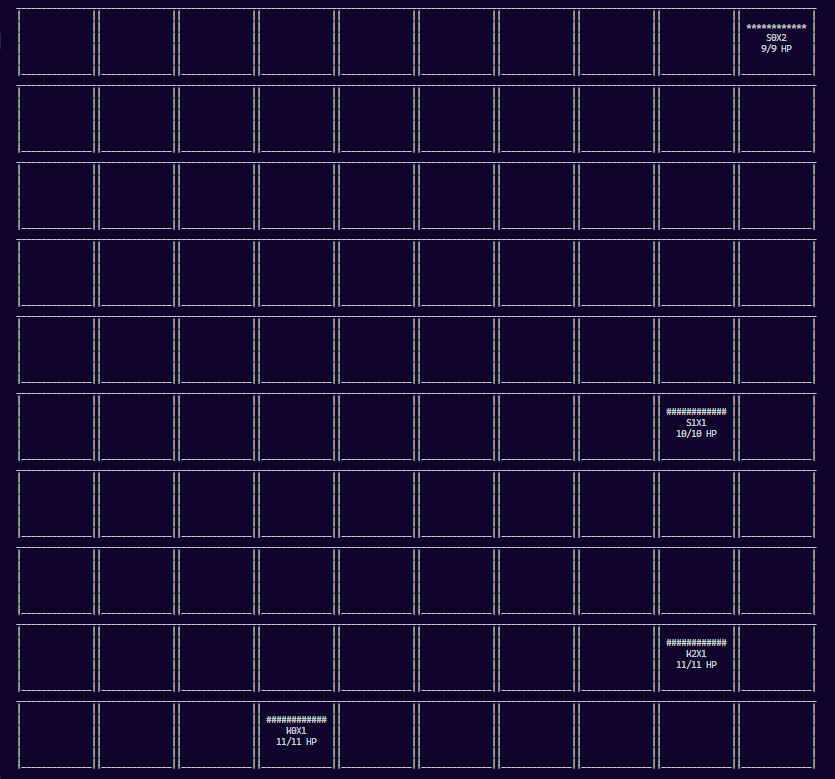
\includegraphics[width=0.6\textwidth,keepaspectratio]{img/tablero.png}
		%\includesvg{img/automata.svg}
		%\label{img:mot2}
		%\caption{Product backlog.}
	\end{figure}
	\begin{itemize}	
		\item Aqui se muestra todo el tablero, mostrando a ambos ejércitos.
	\end{itemize}
	\begin{figure}[H]
		\centering
	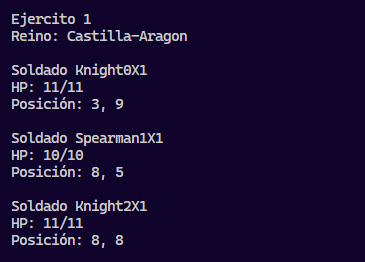
\includegraphics[width=0.6\textwidth,keepaspectratio]{img/mostrar.png}
		%\includesvg{img/automata.svg}
		%\label{img:mot2}
		%\caption{Product backlog.}
	\end{figure}
	\begin{itemize}	
		\item Aqui se muestra el ejército 1, junto a todos sus soldados.
	\end{itemize}
	\begin{figure}[H]
		\centering
	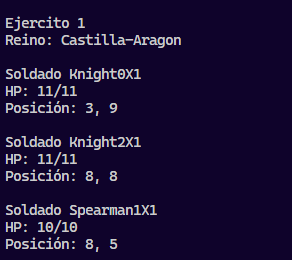
\includegraphics[width=0.6\textwidth,keepaspectratio]{img/ordenar.png}
		%\includesvg{img/automata.svg}
		%\label{img:mot2}
		%\caption{Product backlog.}
	\end{figure}
	\begin{itemize}	
		\item Aqui se muestra el ejército 1, ordenado según vida máxima.
	\end{itemize}
	\begin{figure}[H]
		\centering
	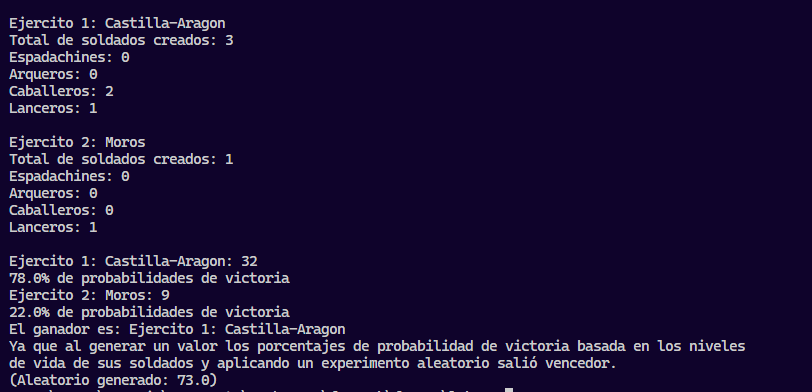
\includegraphics[width=0.6\textwidth,keepaspectratio]{img/resumen.png}
		%\includesvg{img/automata.svg}
		%\label{img:mot2}
		%\caption{Product backlog.}
	\end{figure}
	\begin{itemize}	
		\item Y aquí se ve el resumen realizado al final, que muestra que ejército ganó.
		\item Estos cambios fueron subidos al respositorio, a través de commits.
	\end{itemize}
	
	\begin{lstlisting}[language=bash,caption={Commit}, numbers=left][H]
	$commit db3bba95fe339bfc7101f02caa29bc5f41d0b103 (HEAD -> main, origin/main)
Author: RYAN VALDIVIA <rvaldiviase@unsa.edu.pe>
Date:   Mon Jan 15 00:26:25 2024 -0500

    Creando las clases y metodos necesarios para el funcionamiento principal del videojuego
	\end{lstlisting}
	\begin{itemize}	
		\item Además, aquí está el diagrama UML de todo el proyecto.
	\end{itemize}
	\begin{figure}[H]
		\centering
	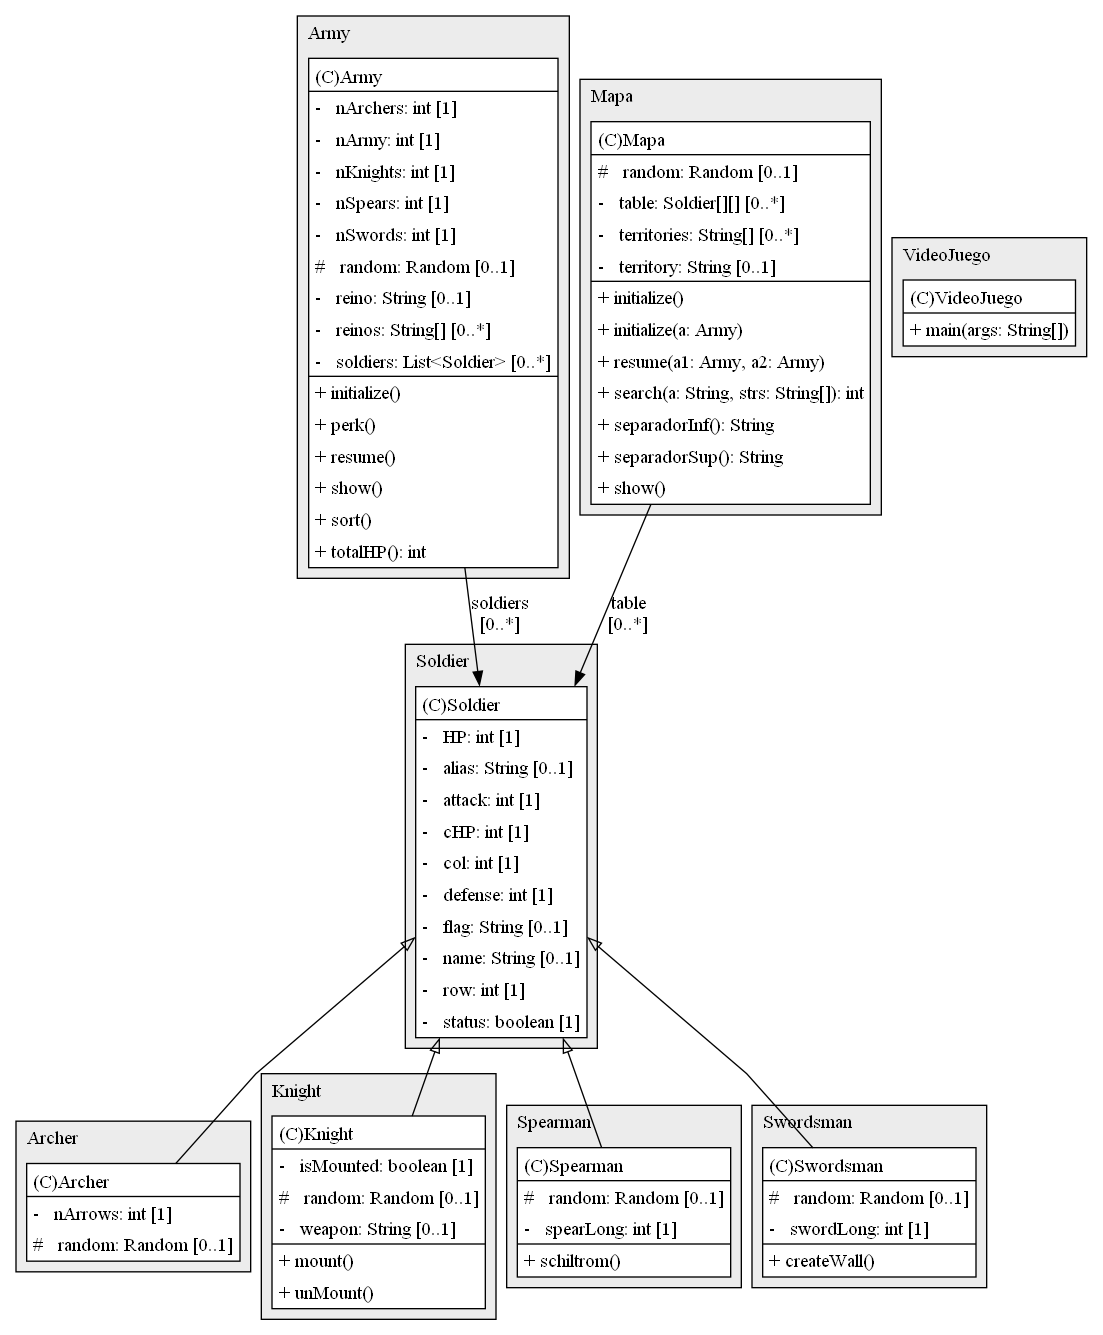
\includegraphics[width=0.6\textwidth,keepaspectratio]{img/VideoJuego_structure.png}
		%\includesvg{img/automata.svg}
		%\label{img:mot2}
		%\caption{Product backlog.}
	\end{figure}
	
	
	\section{\textcolor{red}{Rúbricas}}
	
	\subsection{\textcolor{red}{Entregable Informe}}
	\begin{table}[H]
		\caption{Tipo de Informe}
		\setlength{\tabcolsep}{0.5em} % for the horizontal padding
		{\renewcommand{\arraystretch}{1.5}% for the vertical padding
		\begin{tabular}{|p{3cm}|p{12cm}|}
			\hline
			\multicolumn{2}{|c|}{\textbf{\textcolor{red}{Informe}}}  \\
			\hline 
			\textbf{\textcolor{red}{Latex}} & \textcolor{blue}{El informe está en formato PDF desde Latex,  con un formato limpio (buena presentación) y facil de leer.}   \\ 
			\hline 
			
			
		\end{tabular}
	}
	\end{table}
	
	\clearpage
	
	\subsection{\textcolor{red}{Rúbrica para el contenido del Informe y demostración}}
	\begin{itemize}			
		\item El alumno debe marcar o dejar en blanco en celdas de la columna \textbf{Checklist} si cumplio con el ítem correspondiente.
		\item Si un alumno supera la fecha de entrega,  su calificación será sobre la nota mínima aprobada, siempre y cuando cumpla con todos lo items.
		\item El alumno debe autocalificarse en la columna \textbf{Estudiante} de acuerdo a la siguiente tabla:
	
		\begin{table}[ht]
			\caption{Niveles de desempeño}
			\begin{center}
			\begin{tabular}{ccccc}
    			\hline
    			 & \multicolumn{4}{c}{Nivel}\\
    			\cline{1-5}
    			\textbf{Puntos} & Insatisfactorio 25\%& En Proceso 50\% & Satisfactorio 75\% & Sobresaliente 100\%\\
    			\textbf{2.0}&0.5&1.0&1.5&2.0\\
    			\textbf{4.0}&1.0&2.0&3.0&4.0\\
    		\hline
			\end{tabular}
		\end{center}
	\end{table}	
	
	\end{itemize}
	
	\begin{table}[H]
		\caption{Rúbrica para contenido del Informe y demostración}
		\setlength{\tabcolsep}{0.5em} % for the horizontal padding
		{\renewcommand{\arraystretch}{1.5}% for the vertical padding
		%\begin{center}
		\begin{tabular}{|p{2.7cm}|p{7cm}|x{1.3cm}|p{1.2cm}|p{1.5cm}|p{1.1cm}|}
			\hline
    		\multicolumn{2}{|c|}{Contenido y demostración} & Puntos & Checklist & Estudiante & Profesor\\
			\hline
			\textbf{1. GitHub} & Hay enlace URL activo del directorio para el  laboratorio hacia su repositorio GitHub con código fuente terminado y fácil de revisar. &2 &X &2 & \\ 
			\hline
			\textbf{2. Commits} &  Hay capturas de pantalla de los commits más importantes con sus explicaciones detalladas. (El profesor puede preguntar para refrendar calificación). &4 &X &2 & \\ 
			\hline 
			\textbf{3. Código fuente} &  Hay porciones de código fuente importantes con numeración y explicaciones detalladas de sus funciones. &2 &X &2 & \\ 
			\hline 
			\textbf{4. Ejecución} & Se incluyen ejecuciones/pruebas del código fuente  explicadas gradualmente. &2 &X &2 & \\ 
			\hline			
			\textbf{5. Pregunta} & Se responde con completitud a la pregunta formulada en la tarea.  (El profesor puede preguntar para refrendar calificación).  &2 &X &2 & \\ 
			\hline	
			\textbf{6. Fechas} & Las fechas de modificación del código fuente estan dentro de los plazos de fecha de entrega establecidos. &2 &X &2 & \\ 
			\hline 
			\textbf{7. Ortografía} & El documento no muestra errores ortográficos. &2 &X &2 & \\ 
			\hline 
			\textbf{8. Madurez} & El Informe muestra de manera general una evolución de la madurez del código fuente,  explicaciones puntuales pero precisas y un acabado impecable.   (El profesor puede preguntar para refrendar calificación).  &4 &X &4 & \\ 
			\hline
			\multicolumn{2}{|c|}{\textbf{Total}} &20 & &18 & \\ 
			\hline
		\end{tabular}
		%\end{center}
		%\label{tab:multicol}
		}
	\end{table}
	
\clearpage

\section{Referencias}
	\begin{itemize}
		\item Fundamentos de la programación 2 - Tópicos de la programación Orientada a Objetos (Marco Aedo)
	\end{itemize}
	
%\clearpage
%\bibliographystyle{apalike}
%\bibliographystyle{IEEEtranN}
%\bibliography{bibliography}
			
\end{document}
